\documentclass{standalone}
\usepackage{tikz}
\usepackage{amsfonts, amssymb, amsmath}
\usepackage[dvipsnames]{xcolor}
\usetikzlibrary{3d,calc,patterns,patterns.meta}
\usepackage[export]{adjustbox}


\begin{document}

\begin{adjustbox}{padding=1em}
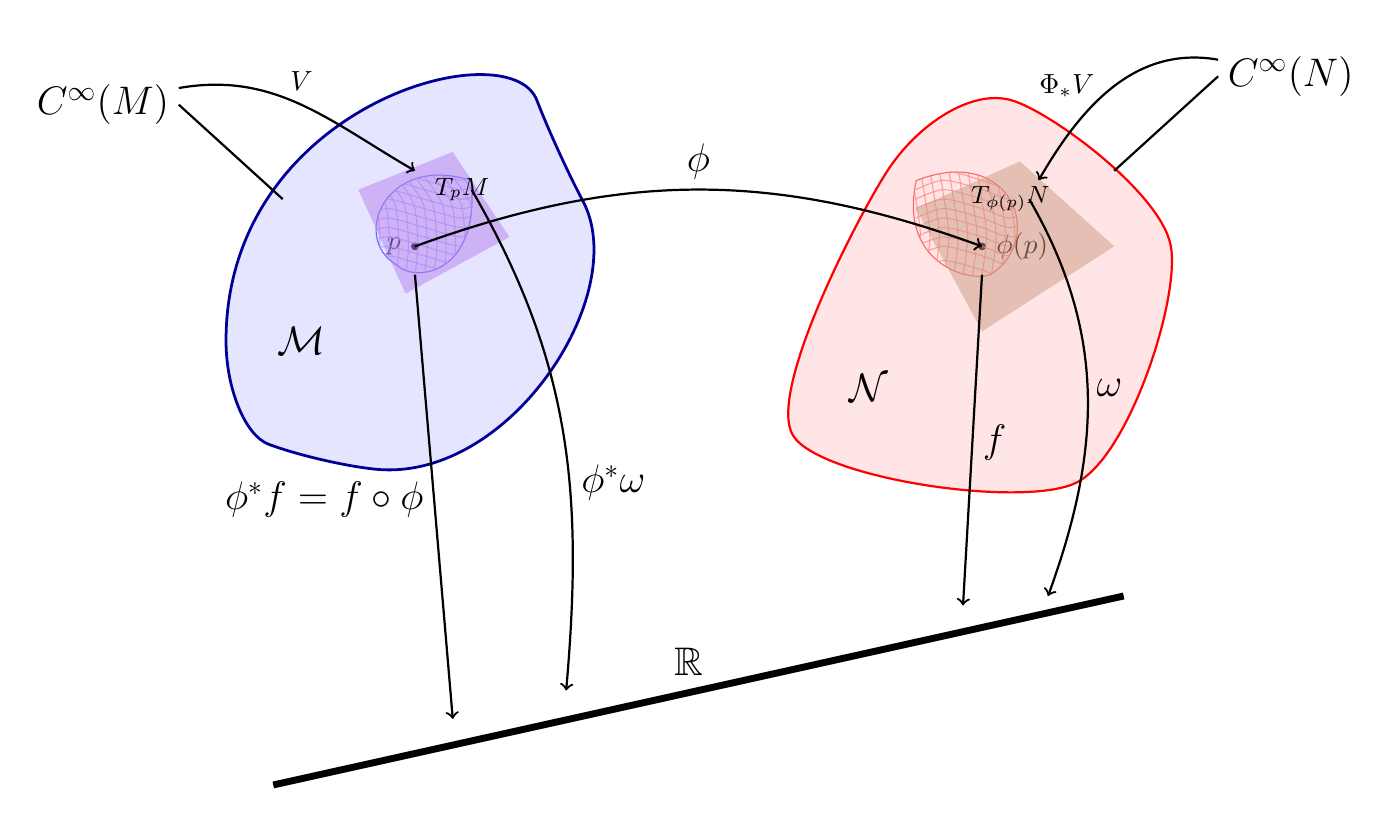
\begin{tikzpicture}[scale=1.2]

% Manifold M (left)
\begin{scope}
  % Shadow near edge
  \path[fill=blue!20, opacity=0.3, rounded corners=20pt]
    (-4,-0.5) .. controls (-4,2) and (-1,2.8) .. (-0.5,1.5)
    .. controls (0.3,0) and (-1,-2) .. (-3,-1.8)
    .. controls (-3.8,-1.5) and (-4,-1) .. (-4,-0.5);

  % Core fill with border
  \draw[fill=blue!10, draw=blue!60!black, line width=1pt, rounded corners=20pt] 
    (-4,-0.5) .. controls (-4,2) and (-1,2.8) .. (-0.5,1.5)
    .. controls (0.3,0) and (-1,-2) .. (-3,-1.8)
    .. controls (-3.8,-1.5) and (-4,-1) .. (-4,-0.5);
  \node at (-3.2,-0.5) {\Large $\mathcal{M}$};
\end{scope}




% Point p on M
\coordinate (p) at (-2,0.5);
\node[circle,fill=black,inner sep=1pt,label=left:$p$] at (p) {};

% Local chart around p (irregular dotted region)
\begin{scope}
  \clip (-1.4,1.2) .. controls (-2.3,1.5) and (-2.7,0.6) .. (-2.2,0.3) .. controls (-2,0.1) and (-1.3,0.2) .. (-1.4,1.2);
  \draw[blue!60, line width=0.8pt]
  (-1.4,1.2) .. controls (-2.3,1.5) and (-2.7,0.6) .. (-2.2,0.3) .. controls (-2,0.1) and (-1.3,0.2) .. (-1.4,1.2);

  % Vertical warped grid lines
  \foreach \x in {-2.6,-2.5,-2.4,...,-1.2} {
    \draw[blue!40, thin, opacity=0.7]
      plot[smooth] coordinates {
        (\x,0.2)
        ({\x+0.03},0.5)
        ({\x},0.9)
        ({\x-0.1},1.1)
        ({\x-0.4},1.5)
      };
  }

  % Horizontal warped grid lines
  \foreach \y in {0.3,0.4,0.5,...,1.4} {
    \draw[blue!40, thin, opacity=0.7]
      plot[smooth] coordinates {
        (-2.6,\y)
        (-2.3,{\y+0.1})
        (-1.9,{\y})
        (-1.5,{\y-0.1})
        (-1.2,\y)
      };
  }
\end{scope}

% Tangent space at p
\fill[BlueViolet!60,opacity=0.5] 
  ($(p) - (0.1,0.5)$) -- 
  ($(p)+(1,0.1)$) -- 
  ($(p)+(0.4,1)$) -- 
  ($(p)+(-0.6,0.6)$) -- 
  cycle;
\node at ($(p)+(0.5,0.6)$) {\small $T_pM$};

% Manifold N (right)
\begin{scope}
\filldraw[fill=red!10, thick, draw=red] plot[smooth cycle] coordinates{(2,-1.5) (5,-2) (6,0.5) (4.3,2.05) (3,1.3)};
\node at (2.8,-1) {\Large $\mathcal{N}$};

\end{scope}

% Point φ(p) on N
\coordinate (phip) at (4,0.5);
\node[circle,fill=black,inner sep=1pt,label=right:$\phi(p)$] at (phip) {};

% Local chart around φ(p)
\begin{scope}
  \clip (3.3,1.2) .. controls (4.3,1.6) and (4.7,0.6) .. (4.1,0.2)
        .. controls (3.9,0.1) and (3.1,0.3) .. (3.3,1.2);
  
  \draw[red!60, line width=0.8pt]
    (3.3,1.2) .. controls (4.3,1.6) and (4.7,0.6) .. (4.1,0.2) .. controls (3.9,0.1) and (3.1,0.3) .. (3.3,1.2);

    % Vertical warped grid lines
  \foreach \x in {3.3,3.4,3.5, ..., 4.5} {
    \draw[red!50, thin, opacity=0.7]
      plot[smooth] coordinates {
        (\x,0.2)
        ({\x+0.05},0.6)
        ({\x},1.0)
        ({\x-0.05},1.3)
      };
  }

  % Horizontal warped grid lines
  \foreach \y in {0.25, 0.4, 0.5, ..., 1.4} {
    \draw[red!50, thin, opacity=0.7]
      plot[smooth] coordinates {
        (3.3,\y)
        (3.6,{\y+0.1})
        (4.0,{\y})
        (4.3,{\y-0.1})
        (4.6,\y)
      };
  }
\end{scope}

% Tangent space at φ(p)
\fill[Sepia!30,opacity=0.5] 
  ($(phip)-(0,0.9)$) -- 
  ($(phip)+(1.4,0.0)$) -- 
  ($(phip)+(0.4,0.9)$) -- 
  ($(phip)+(-0.7,0.4)$) -- 
  cycle;
\node at ($(phip)+(0.3,0.5)$) {\small $T_{\phi(p)}N$};

% Map φ
\draw[->, thick] (p) to[bend left=20] node[above] {\Large $\phi$} (phip);


% ℝ line (horizontal line for codomain)
\draw[-, line width=2.5pt] (-3.5,-5.2) -- (5.5,-3.2); 
\node[draw=none, inner sep=0pt] (real-ax) at(0.9, -3.9) {\Large $\mathbb{R}$};




% Arrows for functions to ℝ
\draw[->, thick] ($(phip)+(0,-0.3)$) -- (3.8,-3.3) node[midway, right, yshift=-1pt] {\Large $f$};
\draw[->, thick] ($(p)+(0,-0.3)$) -- (-1.6,-4.5) node[midway, left, yshift=-1pt] {\Large $\phi^*f = f \circ \phi$};

% Label C^\infty(M)
\draw[-, thick] (-3.4,1.0) -- (-4.5,2.0);
\node[left] at (-4.5,2.0) {\Large $C^\infty(M)$};

% Label C^\infty(N)
\draw[-, thick] (5.4,1.3) -- (6.5,2.3);
\node[right] at (6.5,2.3) {\Large $C^\infty(N)$};

% Arrow from C^\infty(M) to T_pM
\draw[->, thick] ([yshift=5pt] -4.5,2.0) 
  to[out=10, in=150] ($(p)+(0.0,0.8)$);
\node at (-3.2,2.25) {$V$};

% Arrow from C^\infty(N) to T_{φ(p)}N
\draw[->, thick] ([yshift=5pt] 6.5,2.3) 
  to[out=170, in=60] ($(phip)+(0.6,0.7)$);
\node at (4.9,2.2) {$\Phi_*V$};

% Arrow from T_pM to ℝ
\draw[->, thick] ($(p)+(0.6,0.6)$) 
  to[out=-60, in=85] (-0.4,-4.2);
\node at (0.1,-2) {\Large $\phi^*\omega$};

% Arrow from T_{φ(p)}N to ℝ
\draw[->, thick] ($(phip)+(0.5,0.5)$)
  to[out=-60, in=70] (4.7,-3.2);
\node at (5.35,-1) {\Large $\omega$};



\end{tikzpicture}
\end{adjustbox}

\end{document}
